% ---
% Capitulo de revisão de literatura
% ---


\chapter{Referencial Teórico}\label{ch:referencial_teorico}


\section{Autenticação e Identidade}\label{sec:autenticacaoeidentidade}
O problema de estabelecer uma associação entre um indivíduo e uma identidade pode ser dividido em duas categorias: autenticação e identificação~\cite{magalhaes2003biometria}.

\subsection{Autenticação}\label{subsec:autenticacao}
É o processo que verifica a autenticidade de um usuário, processo ou dispositivo.
Essa verificação confirma a legitimidade da entidade em questão.
Durante a autenticação, a parte que examina assegura que a entidade sendo verificada é genuína, e esta última participa ativamente na troca de informações~\cite{usmonov2021identification}.


Para~\cite{conti2017biometric} existem três tipos de autenticação\label{tipos-autenticacao}:

\begin{itemize}
    \item \textbf{Baseada em conhecimento:} utiliza informações que a pessoa sabe, como uma senha.
    \item \textbf{Com base em algo que a pessoa possua}, como um \textit{token} ou cartão inteligente.
    \item \textbf{Com base em características físicas da pessoa}, também conhecidas como biometria.
\end{itemize}


\section{Biometria}\label{sec:biometria}
O termo \("\)biometria\("\) vem das palavras gregas \("\)bios\("\) (vida) e \("\)metrikos\("\) (medida)~\cite{magalhaes2003biometria}.
É o estudo que visa identificar um indivíduo com base em suas características fisiológicas e comportamentais~\cite{handa2019comparative}, ou seja, biometria é uma forma de identificar pessoas usando características físicas ou comportamentais únicas.

Dos tipos mencionados em~\ref{tipos-autenticacao}, a biometria é tida como a abordagem mais segura, já que os atributos físicos de uma pessoa não podem ser furtados, cedidos ou esquecidos.
Falsear a autenticação biométrica é complicado e inviável, uma vez que avalia características singulares do indivíduo~\cite{dos2019tecnologias}.

\subsection{Tecnologias Biométricas}\label{subsec:biometria-tecnologias}

\subsubsection{Reconhecimento facial}\label{subsubsec:reconhecimento-facial}
É uma tecnologia capaz de identificar uma pessoa a partir de uma imagem digital ou de um vídeo, de modo que é comparado as características faciais selecionadas de uma determinada imagem com os rostos existentes num banco de dados~\cite{orvalho2019reconhecimento}.

\begin{longtable}[c]{|l|l|}
    \hline
    \multicolumn{1}{|c|}{\textbf{Problemas}} & \multicolumn{1}{c|}{\textbf{Reconhecimento Facial}} \\ \hline
    \endfirsthead
    \endhead
    Sensor & \begin{tabular}[c]{@{}l@{}}
                 Resolução espacial, taxa\\ de quadros, distância da\\ câmera.
    \end{tabular} \\ \hline
    Envelhecimento & \begin{tabular}[c]{@{}l@{}}
                         Mudanças geométricas\\ entre a infância e a\\ adolescência, rugas e\\ flacidez facial.
    \end{tabular} \\ \hline
    Interação com o usuário & Poses e expressões. \\ \hline
    \begin{tabular}[c]{@{}l@{}}
        Mudanças no meio\\ ambiente
    \end{tabular} & \begin{tabular}[c]{@{}l@{}}
                        iluminação e cena de\\ fundo.
    \end{tabular} \\ \hline
    Outros fatores & \begin{tabular}[c]{@{}l@{}}
                         Maquiagem, acessórios,\\ e oclusão
    \end{tabular} \\ \hline
    \caption*{Fonte: Adaptado de~\cite{usmonov2021identification}}
\end{longtable}



\section{Geolocalização}\label{sec:geolocalizacao}
É o método de identificar a posição geográfica de um objeto, pessoa ou dispositivo eletrônico.
Para isso, utiliza-se de informações provenientes de sinais de \textit{GPS}, torres de celular, endereços \textit{IP} ou redes  \textit{Wi-Fi}.
Em resumo, permite o rastreamento em tempo real da localização de uma entidade~\cite{da2019sistemas}.

\subsection{GPS}\label{subsec:gps}
GPS é sigla da abreviatura de \textit{Global Positioning System}, ou Sistema de Posicionamento Global em português.
Consiste em uma constelação de 24 satélites que orbitam a Terra a uma altitude aproximada de 20.200 km acima do nível do mar.
Essa configuração permite que os receptores determinem sua posição em qualquer lugar do planeta com notável precisão~\cite{el2002introduction}.

\begin{figure}[H]
    \centering
    \caption{Fonte: Sistema de Posicionamento Global (GPS)}
    \begin{minipage}{.9\textwidth}
        \centering
        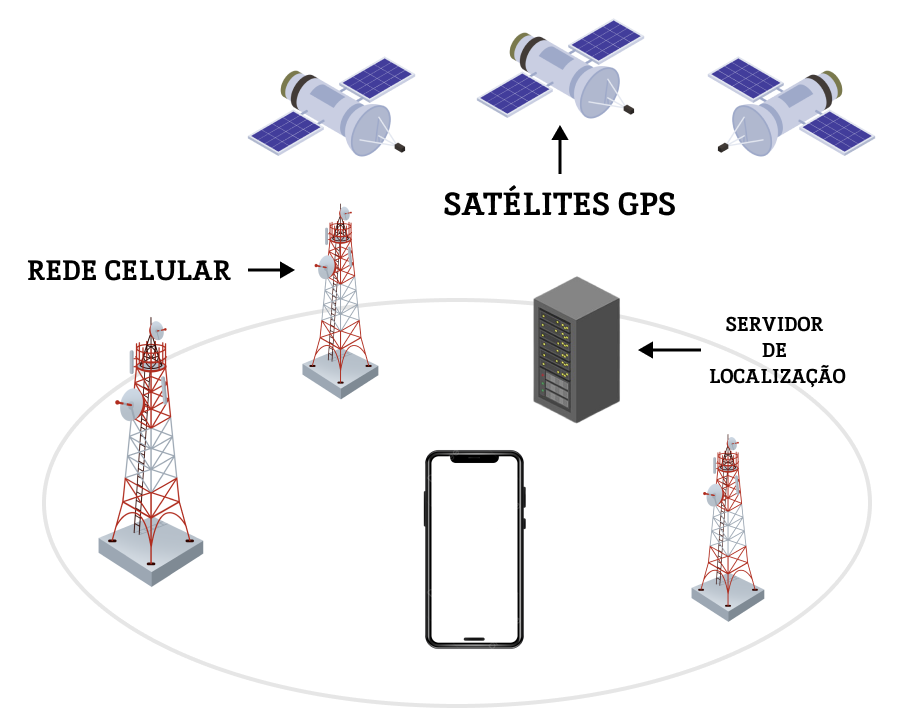
\includegraphics[width=.9\linewidth]{imagens/sistema-gps}
        \label{fig: Sistema de GPS}
    \end{minipage}
    \caption*{Fonte: Adaptada de~\cite{juansyah2015pembangunan}}
\end{figure}

O GPS é o sistema de localização mais popular, cobrindo o mundo inteiro com um erro máximo de 10 metros em áreas abertas.
Esse erro pode ser reduzido a centímetros com uso de tecnicas~\cite{moura2007wbls}.
Esse sistema avançado utiliza uma rede de estações fixas na Terra, que trabalham em conjunto com satélites.
As estações medem a diferença de tempo de chegada dos sinais e, como suas posições são conhecidas, é possível calcular a localização exata através dessa diferença~\cite{djuknic2001geolocation}.

\subsection{Localização Indoor}\label{subsec:localizacao-indoor}

Um dos fatores que aumentam a confiabilidade da localização de uma pessoa ou objeto em um determinado local é o GPS, entretanto, como mencionado em~\ref{subsec:gps}, essa tecnologia apresenta limitações em ambientes fechados.
Quando um receptor está em um espaço interno, torna-se muito difícil decodificar os sinais GPS, uma vez que eles são atenuados por edifícios e paredes.
Isso resulta em perda de potência do sinal e, consequentemente, em erros na localização do receptor.
Nesse contexto, existe a tecnologia de localização indoor, projetada para localizaço em ambientes fechados, como andares de prédios, tuneis, salas ou auditórios~\cite{mittelstadt2018bluepath}.
